\documentclass[11pt,a4paper]{article}
\usepackage[margin=0.85in]{geometry}
\usepackage{amsmath, amssymb}
\usepackage{enumitem}
\usepackage{fancyhdr}
\usepackage{tcolorbox}
\usepackage{mathpazo}
\usepackage{xcolor}
\usepackage{titlesec}
\usepackage{booktabs}
\usepackage{graphicx}
\usepackage{caption}
\usepackage{float}

% Define colors
\definecolor{tumblue}{RGB}{0,101,189}

% Title format
\titleformat{\section}{\large\bfseries\color{tumblue}}{\thesection.}{0.5em}{}
\titlespacing*{\section}{0pt}{1.2ex plus 1ex minus .2ex}{0.5ex plus .2ex}

% Header and Footer
\pagestyle{fancy}
\fancyhf{}
\lhead{\textcolor{tumblue}{\textbf{Deep Learning Seminar, TUM}}}
\rhead{\textit{Lucas Scherberger}}
\cfoot{\thepage}
\renewcommand{\headrulewidth}{0.4pt}
\renewcommand{\headrule}{\hbox to\headwidth{\color{tumblue}\leaders\hrule height \headrulewidth\hfill}}

\captionsetup{font=small,labelfont={bf,color=tumblue}}

\begin{document}

\begin{center}
    \Large \textbf{\textcolor{tumblue}{On the Guidance of Flow Matching: Review on synthetic data}} \\
    \vspace{0.15cm}
    \normalsize \textbf{Speaker:} Lucas Scherberger \hspace{1cm} \textbf{Supervisor:} Lea Zimmermann
\end{center}
\vspace{0.3cm}

\begin{tcolorbox}[colback=tumblue!5!white, colframe=tumblue, title=\textbf{Motivation \& Core Objective}]
\begin{itemize}[leftmargin=*, nosep]
    \item \textbf{Flow Matching (FM):} Generative method learning a velocity field $v_t(x)$ to transport a tractable source distribution $p_0$ into a complex data distribution $p_1$.
    \item \textbf{The Question:} How can we generate \textit{specific parts} of the complex target distribution?
    \item \textbf{Solution:} Energy-based guidance! Steer a frozen model toward a defined objective.
\end{itemize}
\end{tcolorbox}

\section*{1. Notation \& Abbreviations Overview}
\begin{itemize}[leftmargin=*, nosep]
    \item $p_0 \rightarrow p_1$: Source distribution to target data distribution
    \item $v_t(x)$: Learned base velocity field
    \item $J(x)$: Energy function (defines the target subset)
    \item $g_t(x_t)$: Guidance vector field (proportional to $-\nabla J$)
    \item $v' = v_t + g_t$: Guided velocity field
    \item $z = (x_0, x_1)$: Coupling of source and target
    \item $\pi(x_0, x_1)$: Distribution over the source--target coupling
    \item $\mathcal{P}$: Reverse coupling ratio ($\mathcal{P} = 1$ for independent coupling)
\end{itemize}

\section*{2. Steering Mechanisms}
\begin{itemize}[leftmargin=*, nosep]
    \item \textbf{Training-time Steering (Conditioning):} Requires data and a label $y$ during training. The model reproduces seen labels directly.
    \item \textbf{Inference-time Steering (Guidance):} Train the model purely on data. Keep the base flow model frozen. Add guidance $g_t$ at sampling to push the flow toward low energy $J$.
\end{itemize}

\section*{3. Guidance}
\textbf{Guided target distribution.} Guidance reweights the original target $p_1(x)$ by the energy $J$; the subset we want is the low-energy region: $\;p'(x) = \frac{1}{Z}\, p_1(x)\, e^{-J(x)}$.

\noindent\textbf{Guidance vector field} (Theorem 3.1). The field $g_t$ that turns $v_t$ into the guided $v' = v_t + g_t$ is
\begin{equation*}
    g_t(x_t) = \int \left( \mathcal{P}\,\frac{e^{-J(x_1)}}{Z_t(x_t)} - 1 \right) v_{t|z}(x_t|z)\, \underbrace{p(z|x_t)}_{\text{intractable}}\, dz .
\end{equation*}
The intractable posterior $p(z|x_t)$ is what the methods below approximate. \emph{Training-free} methods spend their cost at inference and trade more assumptions for lower cost; the \emph{training-based} method moves the cost to a one-time training.
\begin{itemize}[leftmargin=*, nosep]
    \item \textbf{MC} ($g^{MC}$) -- \textit{training-free, unbiased in the limit.} Monte Carlo estimation of the integral (importance sampling from the prior $p(z)$ instead of the posterior). No gradient of $J$ needed and stays on the data manifold, but has high variance in high dimensions.
    \item \textbf{sim-MC} ($g^{sim\text{-}MC}$) -- \textit{training-free.} Approximates the intractable posterior with a Gaussian and samples from it. Useful when $J$ lacks a clean closed-form expression.
    \item \textbf{cov-A} ($g^{cov\text{-}A}$) -- \textit{training-free, cheapest.} Taylor-expands the guidance locally around the mean (affine path) and replaces the covariance with a hand-set schedule $\lambda_t I$. No extra network evaluations.
    \item \textbf{cov-G} ($g^{cov\text{-}G}$) -- \textit{training-free.} Affine \emph{Gaussian} path: maps FM back to classical diffusion guidance (DPS / $\Pi$GDM) and computes the exact covariance via network Jacobians. Stronger, but costs backprop through the velocity field.
    \item \textbf{GM / Learned} ($g_\phi$) -- \textit{training-based, exact in expectation.} Guidance Matching: trains one network for the normalizing constant $Z$ and a second that directly learns the guidance field. Accurate, at the price of additional training.
\end{itemize}

\section*{4. The Hidden Assumption ($\mathcal{P} \approx 1$)}
\begin{itemize}[leftmargin=*, nosep]
    \item All methods above assume the reverse coupling ratio $\mathcal{P} = \dfrac{\pi'(x_0|x_1)}{\pi(x_0|x_1)} \approx 1$ ($\mathcal{P}=1$ exactly for independent coupling; $\mathcal{P}\approx 1$ whenever $J$ varies slowly).
    \item \textbf{When it breaks:} $g_t$ points in a systematically wrong direction when coupling is \textbf{strong} (e.g.\ exact Optimal Transport) \underline{and} the energy $J$ is \textbf{sharp}. (Quantified in Section~5.)
\end{itemize}

\section*{5. Results (Synthetic Data)}
\textbf{Setup.} A single CFM is trained once on a 2D transport task (e.g.\ Uniform / 8-Gaussian $\rightarrow$ 8-Gaussian, 8-Gaussian $\rightarrow$ Moons), then frozen and steered by an energy $J$ that selects a sub-distribution (here: three of the modes). Guidance methods are compared against unguided CFM and class-conditional CFM (CCFM), which needs the label at training time.

\begin{figure}[H]
    \centering
    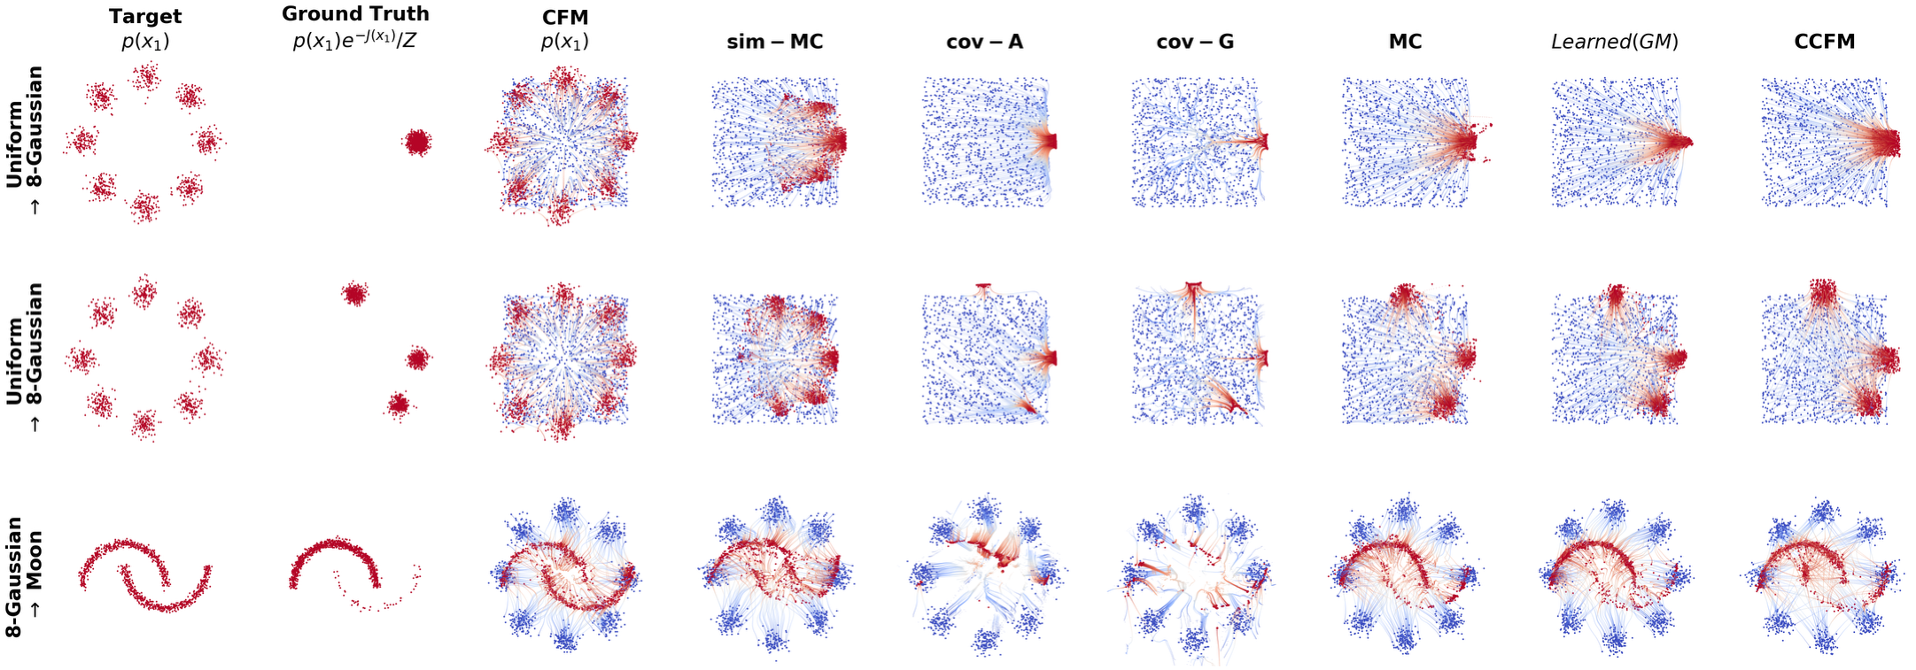
\includegraphics[width=0.88\textwidth]{figs/synthetic_data_three_energy_functions.png}
    \caption{Qualitative comparison. Columns: target $p_1$, ground-truth guided target $p_1 e^{-J}/Z$, unguided CFM, each guidance method, CCFM (last). Learned (GM) and MC reproduce the selected modes most faithfully; gradient-based approximations (cov-A, cov-G, sim-MC) collapse onto points or drift off the data manifold.}
\end{figure}

\noindent\textbf{Takeaways.} Learned (GM) performs best visually and MC stays on the data manifold. Guidance beats the unguided CFM baseline and matches CCFM \emph{without retraining} -- one frozen model generates many sub-distributions, just by changing $J$. A quantitative comparison over four metrics (W2, energy distance, $|1-\text{diversity trace ratio}|$, off-manifold rate) agrees: Learned (GM) and MC are balanced across all four, while unguided CFM is worst.

\noindent\textbf{Where $g^{MC}$ breaks.} The off-manifold rate of $g^{MC}$ (Uniform $\rightarrow$ 8-Gaussian, energy $J$ for three Gaussians) confirms Section~4: failures grow towards \emph{stronger coupling} (left $\to$ right) and \emph{sharper} $J$ (smaller energy width, top of table).

\begin{center}
\renewcommand{\arraystretch}{1.15}
\small
\begin{tabular}{c|cccccc}
\multicolumn{1}{c}{} & \multicolumn{6}{c}{\textbf{Coupling strength (weak $\rightarrow$ strong)}} \\
\textbf{Energy width} & Indep. & Ent.\ $10$ & Ent.\ $1$ & Ent.\ $0.3$ & Ent.\ $0.1$ & Exact-OT \\
\toprule
$0.03$ (sharp) & 0.57 & 0.60 & 0.67 & 0.74 & 0.78 & 0.78 \\
$0.05$         & 0.36 & 0.36 & 0.47 & 0.57 & 0.60 & 0.62 \\
$0.1$          & 0.22 & 0.18 & 0.32 & 0.37 & 0.41 & 0.43 \\
$0.2$ (wide)   & 0.15 & 0.10 & 0.22 & 0.23 & 0.29 & 0.26 \\
\bottomrule
\end{tabular}
\captionof{table}{Off-manifold rate of $g^{MC}$ (lower is better). It climbs towards strong coupling and sharp $J$.}
\end{center}

\section*{6. Conclusion}
\begin{itemize}[leftmargin=*, nosep]
    \item Introduced different guidance methods for conditional flow matching.
    \item Learned (GM) performs slightly better than MC on synthetic data, but at the cost of additional training.
    \item Guidance with $g^{MC}$ under stronger OT coupling and sharp energy functions performs worse.
\end{itemize}

\end{document}